\documentclass[11pt,a4paper,preprint]{aastex}
\usepackage{lscape}
\usepackage{multirow}
\usepackage{rotating}
\usepackage{myaasmacros}
\usepackage{bm}
\usepackage{amsmath}
\usepackage{enumerate}
\usepackage{color}


\usepackage[left=3cm,right=3cm,top=3cm,bottom=3.5cm]{geometry}

\newcommand{\kms}{\mathrm{km}\textrm{ }\mathrm{s}^{-1}}
\newcommand{\kpc}{\mathrm{kpc}}
\newcommand{\Mpc}{\mathrm{Mpc}}
\newcommand{\dd}{\mathrm{d}}
\newcommand{\diag}{\mathop{\mathrm{diag}}}
\newcommand{\udot}{\textrm{ }\dot{}\textrm{ }}
\newcommand{\cc}{(\textrm{c.c.})}
\newcommand{\boxme}[1]{\fbox{\parbox{\textwidth}{#1}}}
\newcommand{\tr}{\mathrm{\mathop{Tr}}}
\newcommand{\lie}{\mathcal{L}}
\definecolor{gray}{RGB}{150,150,150}
\newcommand{\invisible}{\textcolor{gray}}
\setlength{\parindent}{0em}

\newcommand*\colvec[3][]{
    \begin{pmatrix}\ifx\relax#1\relax\else#1\\\fi#2\\#3\end{pmatrix}
}

\newcommand{\bmath}[1]{\ensuremath{\bm{#1}}}
\renewcommand{\vec}[1]{\bmath{#1}}
\newcommand{\tens}[1]{{\bf \sf #1}}
\newcommand{\threej}[6]{{
\left(\begin{array}{ccc} #1 & #3 & #5 \\
 #2 & #4 & #6
\end{array}\right)}}

\newcommand{\D}{\mathcal{D}}

\title{The posterior of a Gaussian subject to $\delta$-function constraints}
\author{Andrew Pontzen}

\begin{document}
\maketitle

Consider a $n$-dimensional Gaussian-distributed data vector $x$, with
mean $\langle \vec{x} \rangle = \vec{x}_0$ and covariance $\langle
(\vec{x}-\vec{x_0})(\vec{x}-\vec{x_0})\rangle = \tens{C}$. The
probabiliy distribution is
\begin{equation}
p(\vec{x}) \propto \exp \left(-\frac{1}{2} (\vec{x} -
  \vec{x}_0)^{\top} \tens{C}^{-1} (\vec{x}-\vec{x}_0) \right)\textrm{,}
\end{equation}
where we have not bothered with normalization (which will be neglected
throughout).

Supose we know that $\vec{x}$ satisfies the linear constraint
$\vec{\alpha}_1 \cdot \vec{x} = d_1$. Then we can legitimately ask
what the new probability distribution $p_1$ is. In fact, this will
turn out to be another Gaussian which means that if we have further
constraints we can simply apply them one-by-one starting from the
original unconstrained distribution.

In the cosmological context, we take a discrete version of our space
(we can use the limit $n \to \infty$ later). We will be constraining
on the smoothed density, $\vec{x}_{\mathrm{smooth}} = \tens{S}_i
\vec{x}$, at some point (say $i=1$ in the vector). Then
$\alpha_i^{\alpha} = S_i^{\alpha \beta} \delta_{\beta}^{1}$. However we
will not need the explicit form whatsoever.

Schematically, we have $p_1(\vec{x}) \propto p_0(\vec{x})
\delta(\vec{\alpha}_1 \cdot \vec{x} - d_1)$. The $\delta$ function
can be approximated as a Gaussian whose width $\beta$ we will allow to
tend to zero later:
\begin{equation}
p_1(\vec{x}) \propto \lim_{\beta \to \infty} p(\vec{x}) \exp \left[
  -\frac{\beta}{2} \left( \vec{\alpha}_1 \cdot \vec{x} - d_1 \right)^2 \right]
\end{equation}

We want to combine the two Gaussians. We assume the new distribution
will have mean $\langle \vec{x} \rangle = \vec{x}_1$ for some
$\vec{x}_1$, and so write
\begin{equation}
p(\vec{x}) \propto \exp \left[-\frac{1}{2} (\vec{x} -
  \vec{x}_1)^{\top} \left(\tens{C}^{-1} + \beta \vec{\alpha}_1
    \vec{\alpha}_1^{\top} \right) (\vec{x}-\vec{x}_1) -
  \vec{x}_1^{\top} \left(\tens{C}^{-1} + \beta \alpha_1
    \alpha_1^{\top} \right) \vec{x} +
  \vec{x}_0^{\top}\tens{C}^{-1}\vec{x} + \beta d_1
  \vec{\alpha}_1^{\top} \vec{x}  \right]
\end{equation}
Here we've thrown away a whole load of terms which are zero-order in
$\vec{x}$ since they just change the normalization. We require the
three dangling linear-in-$\vec{x}$ terms to vanish thus determining
$\vec{x}_1$. We will need two things; first a normalization for the $\vec{\alpha}_1$ which conveniently can
be chosen\footnote{unless $\vec{\alpha}_1$ is a null direction of
  $\tens{C}$, but then there would be zero probability of our
  constraint in the original distribution, so that case is already meaningless. } as 
\begin{equation}
\vec{\alpha}_1^{\top} \tens{C} \vec{\alpha}_1 = 1\textrm{.}\label{eq:norm}
\end{equation}
Second, we'll need the Sherman-Morris formula,
\begin{equation}
(\tens{C}^{-1} + \beta \vec{\alpha}_1 \vec{\alpha}_1^{\top})^{-1} =\tens{C} - \beta \frac{\tens{C} \vec{\alpha}_1 \vec{\alpha}_1^{\top}
  \tens{C}}{1+\beta \vec{\alpha}_1^{\top} \tens{C} \vec{\alpha}_1}
\simeq \tens{C} \left[ 1-(1-\beta^{-1}) \vec{\alpha}_1
  \vec{\alpha}_1^{\top} \tens{C} \right] \textrm{,}
\end{equation}
where I have used $\beta \gg 1$ and the normalization condition
\eqref{eq:norm}.

Then we have
\begin{equation}
\vec{x}_1 = \vec{x}_0 - \left(1-\beta^{-1}\right) \tens{C}
\vec{\alpha}_1 \vec{\alpha}_1^{\top} \vec{x}_0 + \beta \vec{d}_1
\tens{C} \beta^{-1} \vec{\alpha}_1
\end{equation}
and in the limit $\beta \to \infty$,
\begin{equation}
\vec{x}_1 = \left[1-\tens{C} \vec{\alpha}_1 \vec{\alpha}_1^{\top}
\right] \vec{x}_0 + d_1 \tens{C} \vec{\alpha}_1\textrm{.}\label{eq:x1}
\end{equation}
We'll interpret this formula in a moment but first note that 
\begin{equation}
\tens{C}_1 \equiv \left(\tens{C}^{-1} - \beta \alpha_1
  \alpha_1^{\top}\right)^{-1} = \lim_{\beta \to \infty} \tens{C}
\left[1-\frac{\beta \vec{\alpha}_1 \vec{\alpha}_1^{\top}
    \tens{C}}{1+\beta} \right] = \tens{C}
\left[1- \vec{\alpha}_1 \vec{\alpha}_1^{\top}
    \tens{C} \right]\label{eq:C1}
\end{equation}
giving our final updated probability distribution function
\begin{equation}
p(\vec{x}) \propto \exp \left(-\frac{1}{2} (\vec{x} -
  \vec{x}_1)^{\top} \tens{C}_1^{-1} (\vec{x}-\vec{x}_1) \right)\textrm{,}
\end{equation}
with $\vec{x}_1$ and $\tens{C}_1$ given by equation \eqref{eq:x1} and
\eqref{eq:C1} respectively.

The properties of the updated mean and variance are quite
intuitive. The mean ensures that $\vec{\alpha}_1 \cdot \langle \vec{x}
\rangle = d_1$:
\begin{equation}
\vec{\alpha}_1 \cdot \langle \vec{x} \rangle = \vec{\alpha}_1 \cdot
\vec{x}_1 = \vec{\alpha}_1 \cdot \vec{x_0} - \vec{\alpha}_1 \cdot
\vec{x}_0 + d_1 = d_1
\label{eq:newvar}
\end{equation}
where I have used the normalization condition \eqref{eq:norm}.

The covariance ensures that there is no variation along that
direction:
\begin{equation}
0=\langle (\vec{\alpha}_1 \cdot \vec{x}-d_1)^2 \rangle =% \dots =
%\alpha_1^{\top}\tens{C}_1 \alpha_1 -d_1^2 = 0.
\vec{\alpha}_1^{\top}\tens{C}_1 \vec{\alpha}_1 %= 0,
\end{equation}
where we have used \eqref{eq:newvar} in the intermediate steps to cancel all terms which contain $\vec{x}_1$ and $d_1$.

This is a generalized version of Hoffman and Ribak 1991 (ApJ).

To satisfy two constraints, for simplicity on an initially zero-mean
field, start with $\vec{x}_0=0$ and iterate equation \eqref{eq:x1} and
\eqref{eq:C1} twice. The attached program does that and verifies that
the realizations after constraining twice respect both constraints.

If one adds a local density enhancement to a larger scale void, the
void is enhanced in peak depth. This correctly maintains the large scale void at
the same averaged depth. 

\begin{center}
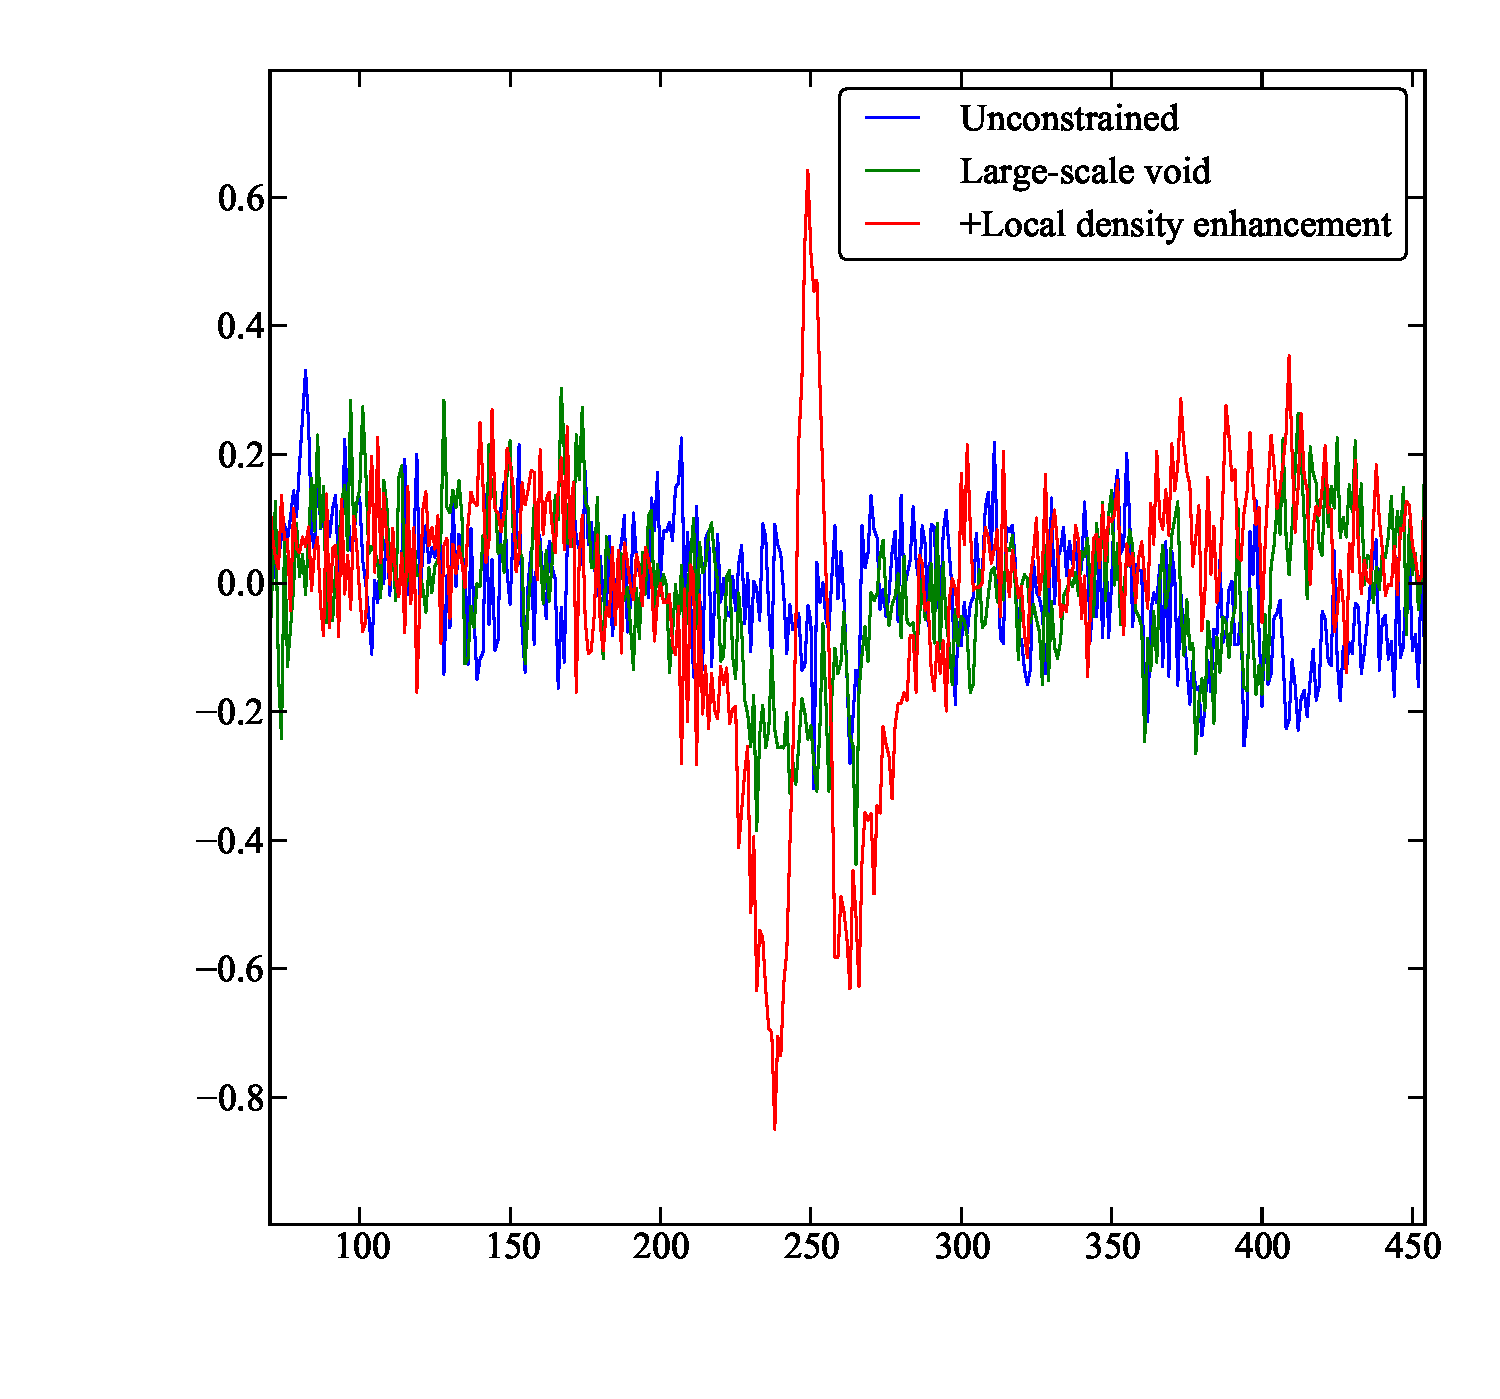
\includegraphics[width=0.5\textwidth]{HR-demo.pdf}
\end{center}


\section{The projection scheme}

Unfortunately the scheme above requires one to sample from the new
covariance matrix $\mathsf{C}_1$. To do that one would need to get the
eigenvalues, and to transform back into a Fourier (or pixel) basis,
also the eigenvectors. This is a horrible problem although Nina made
some progress if we need to go back to it.

Instead if possible let's use an iterative method which works as
follows. The aim is to only ever have diagonal matrices in play. The
strategy is to start with a realization from the original problem --
assumed to be zero mean, covariance $\mathsf{C}$. We can work in
Fourier space so $\mathsf{C}$ is diagonal and multiplication by
$\mathsf{C}$ or $\mathsf{C}^{-1}$ is numerically trivial.

Start by assuming it's possible to get a realization from the
constrained problem by a linear transformation of the unconstrained
problem. Let $\vec{y}_0$ be a realization from the original system and
$\vec{y}_1$ a realization from the constrained system. Then the
assumption is:
\begin{equation}
\vec{y}_1 = (\mathsf{I} + \mathsf{A}) \vec{y}_0 + \vec{x}_1\textrm{,}
\end{equation}
recalling that $\vec{x}_1$ is the mean vector of the new system,
$\vec{x}_1 = d_1 \mathsf{C} \vec{\alpha}_1$. 

Now we can see what condition $\mathsf{A}$ needs to satisfy for us to
get the new covariance correct
\begin{equation}
\langle (\vec{y}_1-\vec{x}_1) (\vec{y}_1-\vec{x}_1)^{\top} \rangle =
\mathsf{C}_1 =
\mathsf{C}_0 - \mathsf{C}_0 \vec{\alpha}_1 \vec{\alpha}_1^{\top} \mathsf{C}_0
\textrm{.}
\end{equation}
using equation \eqref{eq:C1} above.

\subsection{November 2014 - the new scheme}

To solve this, we can just set
\begin{equation}
\mathsf{A} = - \mathsf{C}_0 \alpha_1 \alpha_1^{\dagger}\textrm{,}
\end{equation}
which gives
\begin{align}
\mathsf{C}_1 & = (\mathsf{I} - \mathsf{C}_0 \alpha_1
\alpha_1^{\dagger}) \mathsf{C}_0  (\mathsf{I} - \alpha_1
\alpha_1^{\dagger} \mathsf{C}_0 ) \\
& = \mathsf{C}_0 - 2 \mathsf{C}_0 \alpha_1 \alpha_1^{\dagger}
\mathsf{C}_0 + \mathsf{C}_0 \alpha_1 \alpha_1^{\dagger}
\mathsf{C}_0 \alpha_1 \alpha_1^{\dagger}
\mathsf{C}_0  \\
& = \mathsf{C}_0 - \mathsf{C}_0 \alpha_1 \alpha_1^{\dagger}
\mathsf{C}_0\textrm{ as required,}
\end{align}
where I have used the normalization condition \eqref{eq:norm}.

\subsection{The old iterative scheme}
 We now make two ansatz, first that
$\mathsf{A} = \mathsf{C}_0 \tilde{\mathsf{A}}$, second that $\mathsf{A} =
\mathsf{A}^{\top}$. [The first can always be made since $\mathsf{C}_0$
is invertible; the second is slightly less clear, but presumably we'd
reach a contradiction if it was invalid? Perhaps this needs a little
thought, but in practice the following works so it must be fine!]

With this transformation, we get the following equation for $\tilde{\mathsf{A}}$:
\begin{equation}
2 \tilde{\mathsf{A}} + \tilde{\mathsf{A}} \mathsf{C}_0
\tilde{\mathsf{A}} = - \vec{\alpha}_1 \vec{\alpha}_1^{\top}  
\end{equation}
This is a quadratic equation in the matrix $\tilde{\mathsf{A}}$, which
are generically hard things to solve analytically. However there is an
iterative numerical solution. Namely let us start with the solution
ignoring the quadratic correction,
\begin{equation}
\tilde{\mathsf{A}}_0 = -\frac{1}{2} \vec{\alpha}_1 \vec{\alpha}_1^{\top}\textrm{.}
\end{equation}
(For avoidance of doubt, note the numbering on $\tilde{\mathsf{A}}$ is
not going to count the number of applied constraints like numbering
was earlier on, it's going to count the number of iterations.) Then to
get $\tilde{\mathsf{A}}_{i}$ we apply the formula
\begin{equation}
\tilde{\mathsf{A}}_{i} = -\frac{1}{2} \left(\tilde{\mathsf{A}}_{i-1}
  \mathsf{C}_0 \tilde{\mathsf{A}}_{i-1} + \vec{\alpha}_1 \vec{\alpha}_1^{\top} \right)\textrm{.}
\end{equation}
As written, there are a whole load of matrix operations that we wanted
to avoid! However, suppose we have an algorithm ${\tt calculateA(i-1,z)}$
that calculates $\tilde{\mathsf{A}}_{i-1} \vec{z}$ for any vector
$\vec{z}$, without calculating the enormous matrix
$\tilde{\mathsf{A}}_i$. Then we can write down the algorithm for ${\tt
  calculateA(i,z)}$ as
\begin{equation}
{\tt calculateA(i,z) = -0.5 \left(calculateA(i-1, C_0 \cdot calculateA(i-1,
  z)) + \vec{\alpha}_1 \vec{\alpha}_1^{\top} \vec{z} \right)}\textrm{.}
\end{equation}
Note this algorithm uses only matrix multiplication by $\mathsf{C}_0$
(which is diagonal) and vector dot products. So it is tractable even
for huge $N$! 

Then the actual result we want is
\begin{equation}
\vec{y}_1 = \vec{y}_0 + \mathsf{C}_0 \cdot {\tt
  calculateA}(N_{iter},\vec{y}_0) + \vec{x}_1
\end{equation}
where $N_{iter}$ is the total number of iterations. The computational
complexity scales as $N_{iter}^2$, because of the nested calls to {\tt
  calculateA}. But the memory requirements are constant with
$N_{iter}$ (and, when implemented correctly, scale only with the
number of particles, since one never has to store a matrix). I find
$N_{iter}=5$ is plenty for simple 1D test problems.

A demo is provided as {\tt demo2} in the attached program. Here, I
constrain the spatial average value in some region (much like for the
original demo of the basic H-R procedure). The top panels show the
output covariance matrices, from left to right these are
\begin{itemize}
\item The actual exact $\mathsf{C}_1$ calculated from equation
  \eqref{eq:C1} (it's tractable for these test problems of course)
\item The estimate of $\mathsf{C}_1$ from 10\,000 direct realisations,
  showing the level of numerical noise (which goes down with sqrt of
  the number of realisations)
\item The estimate of $\mathsf{C}_1$ from 10\,000 realisations
  calculated using the iterative algorithm, with $N_{iter}=5$. It
  looks like the noise here is pretty consistent with that just from
  the realisation noise, as above.
\item The same, with $N_{iter}=0$. 
\end{itemize}

The bottom panels show the errors in the covariance matrix
estimates. For $N_{iter}=5$, these are consistent with just coming
from the realisation noise. For $N_{iter}=0$ there are clearly still
systematic errors (unsurprising!) but the point is you don't need too
many iterations to converge to the right answer.

All in all, I'd have to say this is pretty nice stuff. Mathematics, eh?

\begin{center}
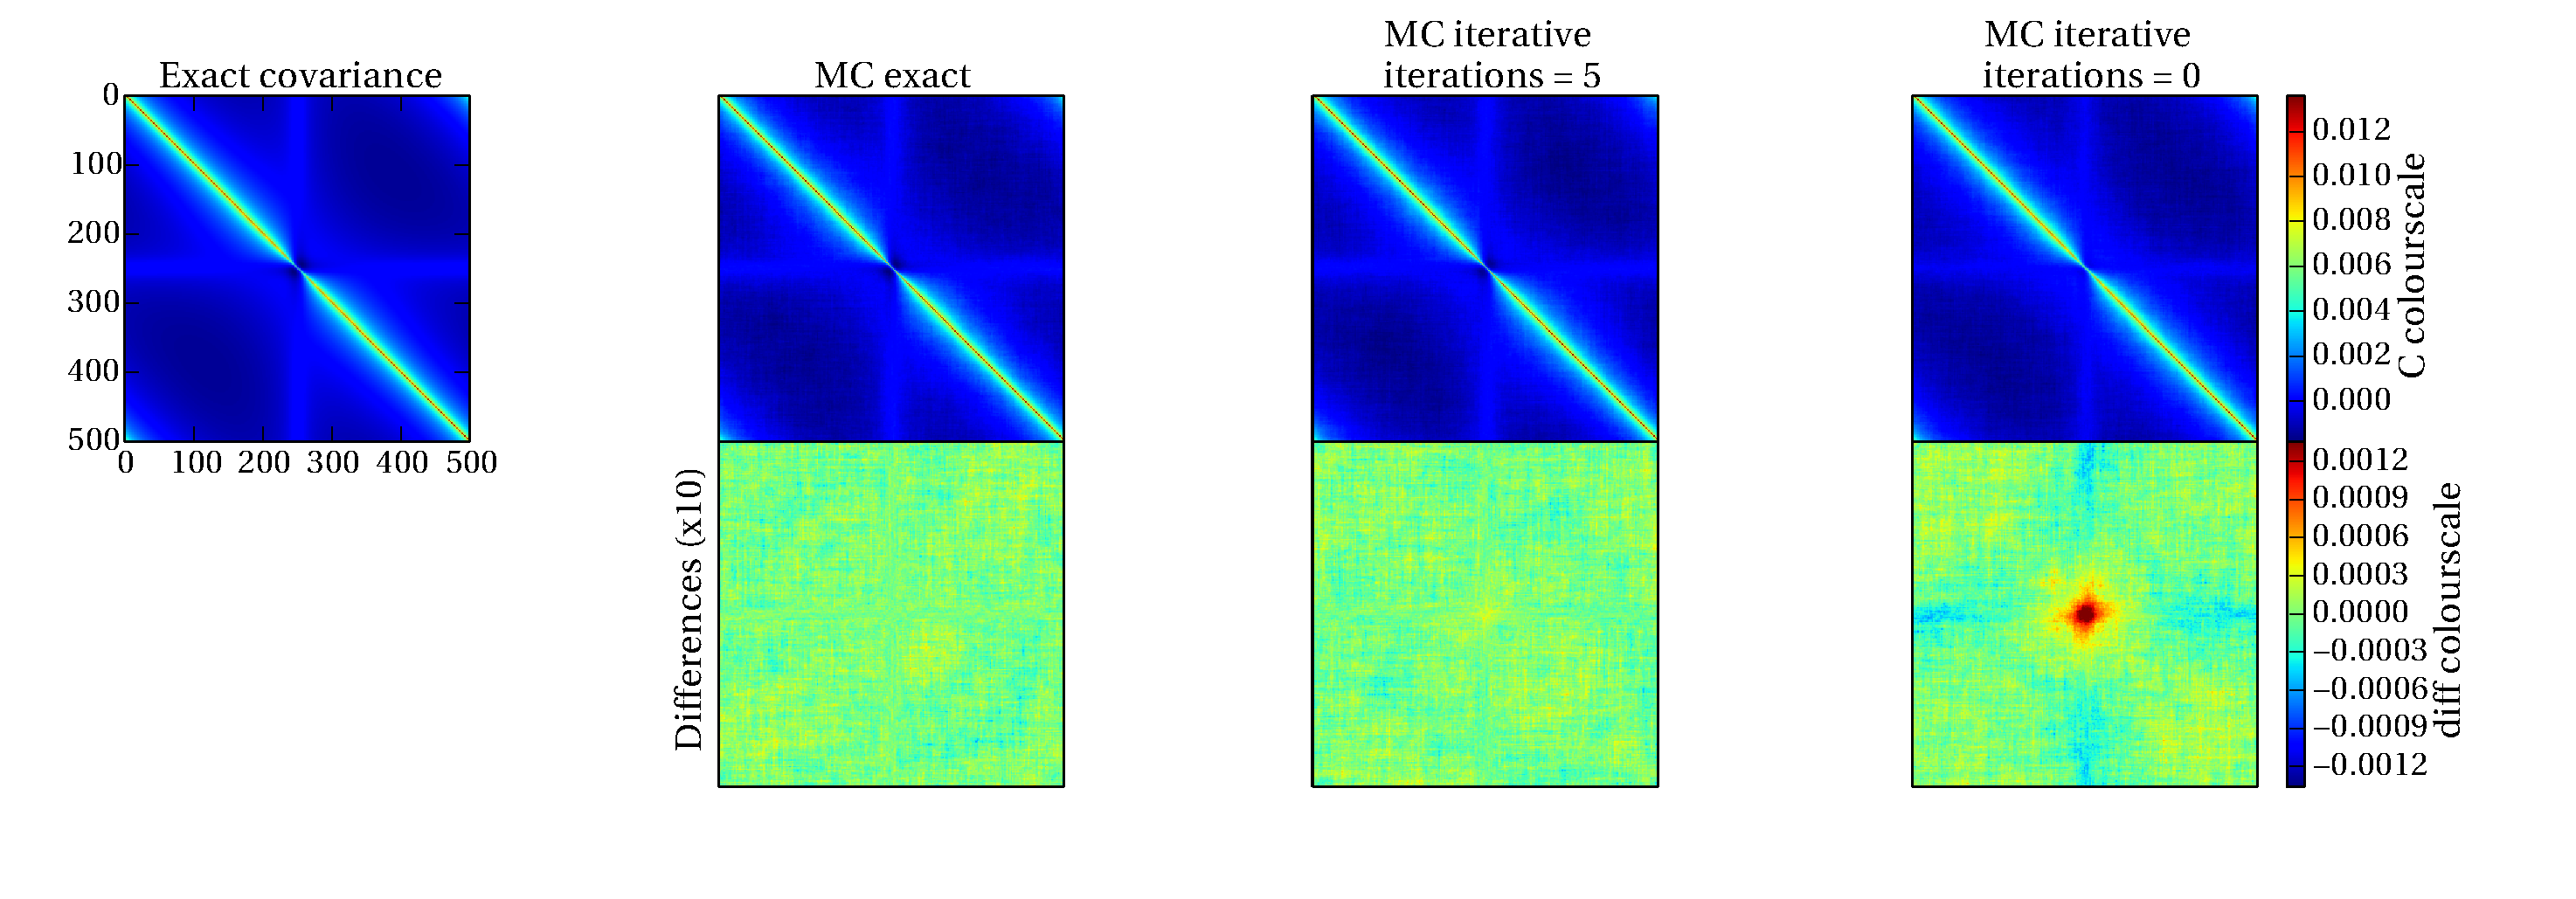
\includegraphics[width=1.1\textwidth]{HR-approx-demo.pdf}
\end{center}

\section{Angular momentum constraints}
\label{sec:AM}

Instead of constraining $\delta$, we actually want to constrain the angular momentum. Fortunately, the method detailed above can be rather straightforwardly extended to do this. 

First of all we note that the constraint condition
\begin{equation}
d= \vec{\alpha} \cdot \vec{\delta}
\end{equation}
is equivalent to 
\begin{equation}
d= \vec{\alpha}^{\mathrm{P}} \cdot \vec{\phi}
\end{equation}
where $\vec{\delta}$ and $\vec{\phi}$ (the potential) are related via the Poisson equation, and $\vec{\alpha}$ and $\vec{\alpha}^{\mathrm{P}}$ by its inverse.

To linear order, the angular momentum of a set of particles is given by
\begin{equation}
L_{\mu} \propto - \sum_j \sum_{\nu, \rho} \epsilon_{\mu \nu \rho} \vec{x}_j^{\nu} \left[ \partial_{\rho} \vec{\phi} \right] _j
\label{eq:L}
\end{equation}
where Roman indices sum over a set of particles and Greek indices sum over the 3 spatial directions. The final term therefore represents the derivative in direction $\rho$ at position $\vec{x}_j$. We can rewrite this term as a finite difference (here: 4th order)
\begin{equation}
\left[ \partial_{\rho} \vec{\phi} \right] _j =  \partial_{\rho} \phi(\vec{x})|_{\vec{x}=\vec{x}_j} = a \vec{x}_j^{\rho-2} +b\vec{x}_j^{\rho-1} -b \vec{x}_j^{\rho+1} -a \vec{x}_j^{\rho+2}
\end{equation}
where $\vec{x}_j^{\rho+s}$ means the coordinate obtained by shifting of $\vec{x}_j$ by $s$ grid cells in direction $\rho$, $a=1/(12 \Delta) $, $b=-2/(3 \Delta)$, and $\Delta$ is the grid spacing.

If we then require the constrained field to obey
\begin{equation}
L_{\mu} = \vec{\alpha}_{\mu}^{\mathrm{P}} \cdot \vec{\phi},
\label{eq:Lconst}
\end{equation}
we can find the components of $\vec{\alpha}_{\mu}^{\mathrm{P}}$ by comparing terms between the right-hand-sides of equations (\ref{eq:L}) and (\ref{eq:Lconst}). Note that the sum over $j$ in Equation (\ref{eq:L}) can go over an arbitrary number of particles, while the scalar product in Equation (\ref{eq:Lconst}) implies a sum over all grid points. Some components of $\vec{\alpha}^{\mathrm{P}}$ receive contributions from multiple particles, while others may be 0.

After numerically calculating $\vec{\alpha}_{\mu}^{\mathrm{P}}$, we can get the usual $\vec{\alpha}_{\mu}$ from the inverse Poisson equation and iteratively constrain the density field as detailed in the previous section. 
One difference here is that there are now technically three constraint vectors, one for each component of $L_{\mu}$, which are not independent of each other (in the sense that $\vec{\alpha}_i$ may get contributions from each direction). Other directions can be constrained by using linear combinations of these $\vec{\alpha}_{\mu}$. However, this also means that even if one chooses a "pure" constraint vector in only one direction, the angular momentum in the other directions will also change.
\end{document}
